\documentclass[fontsize=11pt, a4paper, ngerman]{scrartcl}

\usepackage[theme,typo,icons,aufgaben]{arbeitsblatt}
\aboptionen{
	name={J. Neugebauer},
	kuerzel=Ngb,
	titel={Die CAESAR-Chiffre},
	reihe={Kryptografie},
	fach={Informatik},
	lerngruppe={Q2-GK},
	nummer={III.1},
	lizenz={cc-by-nc-sa-4},
	version={2020-01-08},
}

\usetikzlibrary{shapes}

\begin{document}
\ReiheTitel

Bei der CAESAR-Verschlüsselung werden die Buchstaben des Alphabets (zunächst
nur Großbuchstaben) um eine feste Anzahl an Stellen verschoben. Bei einer
Verschiebung um 3 Stellen wird zum Beispiel aus einem \texttt{B} ein \texttt{E},
usw. Die Verschiebung kann auch als Buchstabe dargestellt werden. Im obigen
Fall ist der Schlüsselbuchstabe \texttt{D}, da bei einer Verschiebung um 3
Stellen der Buchstabe \texttt{A} zu \texttt{D} wird.

\begin{aufgabe}
	Chiffriere das Wort \texttt{KLARTEXT} durch das CAESAR-Verfahren mit dem
	Schlüsselbuchstaben \texttt{G}.
\end{aufgabe}

\begin{aufgabe}
	Die drei Geheimtextnachrichten wurden mit dem CAESAR-Verfahren verschlüsselt.
	Die verwendeten Schlüssel sind auch angegeben, aber durcheinander geraten.

	\begin{center}
	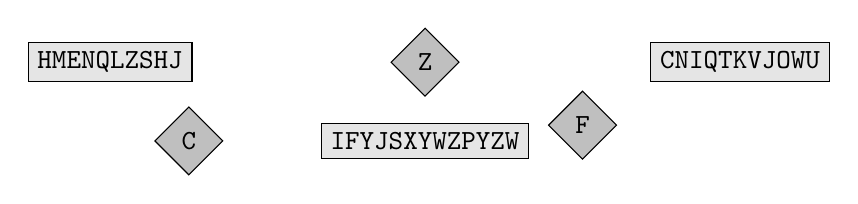
\begin{tikzpicture}[every node/.style={font=\ttfamily}]
		\node[draw,fill=black!10] at (0,0) {HMENQLZSHJ};
		\node[draw,fill=black!10] at (8,0) {CNIQTKVJOWU};
		\node[draw,fill=black!10] at (4,-1) {IFYJSXYWZPYZW};

		\node[draw,fill=black!25,diamond] at (1,-1) {C};
		\node[draw,fill=black!25,diamond] at (4,0) {Z};
		\node[draw,fill=black!25,diamond] at (6,-.8) {F};
	\end{tikzpicture}
	\end{center}

	Ordne die Schlüssel den Geheimtexten zu und entschlüssele die Botschaften.
\end{aufgabe}

\begin{aufgabe}
	Verschlüssele ein Wort oder einen Satz mit dem CAESAR-Verfahren. Tausche die
	verschlüsselte Botschaft dann mit einem Mitschüler/einer Mitschülerin aus, \emph{aber
	nicht die Schlüssel}.

	Versucht nun jeweils die erhaltene Botschaft zu entschlüsseln.
\end{aufgabe}

\begin{aufgabe}
	Verfasst gemeinsam einen Algorithmus (Pseudocode), mit dem das CAESAR-Verfahren geknackt
	werden kann (also entschlüsseln, ohne das Schlüsselwort zu kennen).
\end{aufgabe}

\end{document}
